\chapter{Background and Related Work} % (fold)
\label{chap:Background and Work}


\section{Multicast Protocols} % (fold)
\label{sec:Mutlicast Protocols}
Multicast communication refers to the simultaneous delivery of data towards an
    arbitrary number of destinations
    \cite{mc_routing_multimedia, mc_comm_multicomputer}.
Numerous network protocols have been developed to facilitate multicast
communication, encompassing both Network Layer as well as Application Layer
    implementations \cite{universal_mc, overlay_mc_routing}.
This chapter first distinguishes Multicast from other communication schemes.
Subsequently, various multicast protocols are introduced.

According to the OSI model \cite{osi1980} Layer 3, known as the Network Layer,
    is responsible for end-to-end delivery of data between nodes.
In computer networks data is transferred through \glspl{pdu}, composed of
    protocol specific control information (e.g. source and destination
    address), along with a payload carrying the actual data.
To establish a path from the sender to the destination(s), packets (Layer 3
    \glspl{pdu}) may traverse multiple intermediate nodes \cite{rfc791_ip}.
This process is called routing and can be classified into various schemes.
For the purpose of this thesis, our primary focus lies on the schemes depicted
    in \autoref{fig:multicast}.
\textit{Unicast} denotes a one-to-one association between a sender and a single
    destination.
\textit{Broadcast} disseminates packets to all nodes within the sender's
    broadcast domain (Layer 2) \cite{broadcast}.
Typically, IP Routers (Layer 3) serve as the boundary of a broadcast domain.
\textit{Multicast} transmits packets to a group of destinations, accommodating
    both one-to-many and many-to-many communication \cite{rfc1112_ip4mc}.
In contrast to Broadcast, Multicast does not necessarily deliver packets to all
    available nodes.
Furthermore, Multicast packets can be delivered beyond the sender's broadcast 
    domain, implying subsequent replication of the packets.

% This layer is responsible for end-to-end delivery of data between nodes across
%     interconnected networks.
% A network comprises interconnected nodes, each assigned a unique address within
%     this network \cite{rfc791_ip}. 
% Data delivery is achieved through the transmission of network packets,
%     consisting of a header containing the source and destination address, along
%     with a payload carrying the actual data.
% If the data size exceeds the maximum transfer unit of Layer 2, it is fragmented
%     into multiple packets and subsequently reassembled.

\begin{figure}[h]
    \begin{center}
        \includegraphics[width=0.85\textwidth]{multicast.pdf}
    \end{center}
    \caption{Network Layer: Routing schemes}
    \label{fig:multicast}
\end{figure}


\subsection{IP Multicast} % (fold)
\label{sub:IP Multicast}
Already in the late 1980s, \citeauthor{deering1990multicast}
    \cite{deering1990multicast} proposed an extension to the IP protocol, to
    facilitate efficient multipoint communication (\textit{1:n}, \textit{m:n}).
This extension is known as IP-Multicast and was first standardized in RFC 988
    (\citeyear{rfc988_initmc}) \cite{rfc988_initmc}.
IP-Multicast offers the advantage, to greatly reduce the bandwidth by condensing
    identical traffic into a single stream targeted to a so called ``Host
    Group'' \cite{rfc1112_ip4mc}.
IP-Multicast operates on a separate address space and host groups are
    identified based on an IP address within the designated address range.
For instance, IPv4 host groups are identified by class D IP addresses starting
    with ``\texttt{1110}'' as their \glspl{msb} \cite{rfc1112_ip4mc}.
This characteristic facilitates high scalability, such that host groups may
    encompass thousands of receivers, since senders are not required of any
    knowledge about the number of receivers nor receivers identity or location.
Intermediate nodes like IP routers replicate multicast packets addressed to an
    host group where the paths towards the receivers diverge.
\begin{itemize}\itemsep0em
    \item Separate address space
    \item IGMP / MLD
    \item Intra-Domain Routing: DVMRP, MOSPF, PIM dense/spare
    \item Inter-Domain Routing: MBGP, MSDP
\end{itemize}
% subsection IP Multicast (end)


% \subsection{Multicast over Unicast} % (fold)
% \label{sub:Multicast over Unicast}
% \begin{itemize}\itemsep0em
%     \item Xcast family (Xcast, Xcast+, GXcast, Xcast6 Treemap (island))
%     \item MEADcast
%     \item Bier
% \end{itemize}

\subsection{Explicit Multicast}
\label{sub:Xcast}
Traditional multicast protocols excel in scaling with large multicast groups
    but face challenges with a high number of distinct groups.
\gls{xcast}, on the other hand, is a multicast protocol with complementary
    scaling properties compared to the traditional approach \cite{xcast_rfc}.
\gls{xcast} is designed to efficiently support a vast number of small multicast
    sessions by encoding receiver addresses explicitly in each packet instead
    of relying on multicast addresses \cite{xcast_rfc}.
Furthermore, \gls{xcast} eliminates the necessity for per-session signaling and
    per-session state information, which are characteristic of IP Multicast.
The sender encodes the list of destinations in the \gls{xcast} header and
    transmits the packet to a router.
Upon receiving the packet, each router along the path processes the header, 
    partitions the destinations based on their next hop and forwards a packet
    with a corresponding \gls{xcast} header to each next hop \cite{xcast_rfc}.
When only one destination remains for a next hop, the \gls{xcast} packet can be
    transformed into an IP Unicast packet, a process referred to as \gls{x2u}
    \cite{xcast_rfc}.

In the example illustrated in \autoref{fig:xcast}, the sender $S$ transmits
    data to receivers $E_1$, $E_2$, and $E_3$.
Consequently, $S$ transmits a \gls{xcast} packet to router $R_1$:
    \mintinline{text}{{src=S, dst={E1, E2, E3}}}.
Upon receiving an \gls{xcast} packet, a router process the header as
    follows: \cite{xcast_rfc}
(1) Perform a routing table lookup for each destination listed in the packet
    to determine their next hop.
(2) Group the destinations based on their next hops.
(3) Create a replica of the packet for each next hop.
(4) Modify the destination list of each replica to inclide only the
    destinations that should be routed through that next hop.
(5) Send each replica to its respective next hop.
(6) If only one destination remains for a next hop, perform a \gls{x2u}.

In the scenario demonstrated in \autoref{fig:xcast}, router $R_1$ sends a
    single \gls{xcast} packet with a destination list of
    \{$E_1$, $E_2$, $E_3$\} to $R_2$.
Router $R_2$ sends a replica with a destination list of \{$E_2$, $E_3$\} to
    $R_4$ and performs a \gls{x2u}, transmitting an IP Unicast packet to $R_3$.
$R_3$ forwards the IP Unicast packet as usual to receiver $E_1$.
$R_4$ forwards the packet to router $R_5$ without creating any replicas.
When the packet reaches $R_5$, \gls{x2u} are performed for both $E_2$ and
    $E_3$, and the resulting packets are forwarded accordingly to $R_6$ and
    $R_7$.
Finally, routers $R_6$ and $R_7$ forward default IP Unicast packets to $E_2$
    and $E_3$, respectively.

\begin{figure}
    \centering
    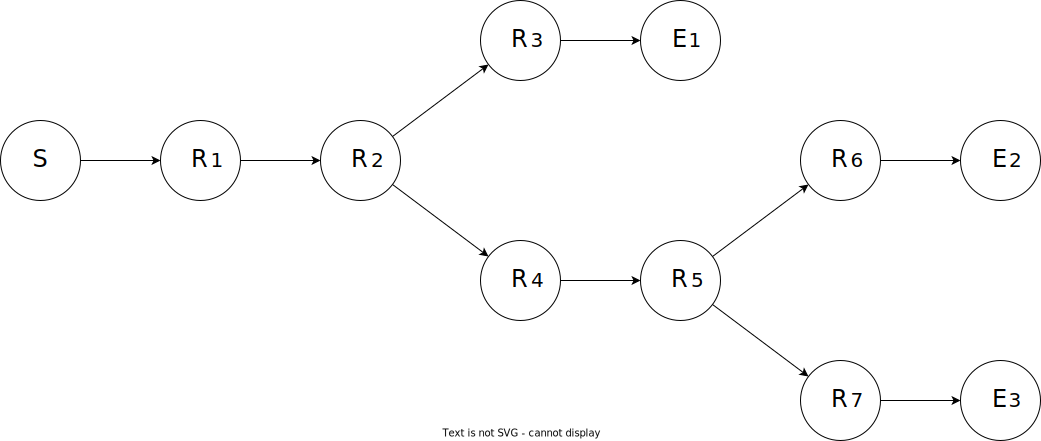
\includegraphics[width=.75\textwidth]{Bilder/xcast.pdf}
    \caption{Xcast processing (based on \cite{xcast_rfc})}
    \label{fig:xcast}
\end{figure}

For IPv6 \gls{xcast} is encoded in the routing extension header, optionally
    followed by a destination extension header specifying a port list,
    particularly in cases where receiver ports are diverging \cite{xcast_rfc}.
The IP destination field carries the \textit{``All-Xcast-Routers''} multicast
    address, necessitating  each \gls{xcast} router to join this multicast
    group.
As a result, each router is required to support \gls{xcast}.
For a gradual deployment, tunnel connections must be established between
    \gls{xcast} routers.
Alternatively, a tunnel connection can assembled to one \gls{xcast}-aware
    receiver.
This receiver has the capability to forward the packet either as an \gls{xcast}
    or IP unicast packet to the remaining endpoints \cite{xcast_rfc}.
% subsection Xcast (end)

\subsection{Explicit Multicast Extension} % (fold)
\label{sub:Explicit Multicast Extension}
There are several extensions to \gls{xcast}, one of which is known as
    \gls{xcast+} \cite{xcast+}.
A key enhancement of \gls{xcast+} is the reduction of the header overhead
    through the introduction of \glspl{dr} \cite{xcast+}.
The router nearest to a receiver determines itself as its \gls{dr}.
A client initiates the session by sending an IGMP ($S$, $G$) message ($S$:
    sender address, $G$: group address) to its \gls{dr}.
Upon receiving, the \gls{dr} sends a so-called \gls{xcast+} registration
    request message encompassing the sender's address ($S$), group address
    ($G$), and its own address towards the sender.
When the \gls{dr} at the sender's side receives it, it keeps track of all the
    \gls{dr} addresses interested in the multicast session ($S$, $G$).
When the sender transmits a multicast packet to its corresponding \gls{dr},
    it explicitly encodes the addresses of the \glspl{dr} at the receivers'
    side in the \gls{xcast} header and transmits the \gls{xcast+} packet, a
    process referred to as \gls{m2x}.
Consequently, \glspl{dr} are not stateless anymore.
Upon receiving \gls{xcast} packets, they perform a so-called \gls{x2m}
    transformation.
As a result, the corresponding address list of \gls{xcast+} might be
    significantly shorter compared to its \gls{xcast} alternative.

For instance in the scenario depicted in \autoref{fig:xcast}, $E_1$, $E_2$, and
    $E_3$ send an IGMP join message ($S$, $G$) to their respective \glspl{dr}
    $R_3$, $R_6$, and $R_7$.
Upon receiving, the receivers' side \glspl{dr} $R_3$, $R_6$, and $R_7$ send an
    \gls{xcast+} registration request ($S$, $G$, $R_i$) towards sender $S$.
When the \gls{dr} on the sender side receives the \gls{xcast+} registration
    requests, it adds a tuple for $R_3$, $R_6$, and $R_7$ encompassing ($S$,
    $G$, $R_i$) to its \gls{xcast+} table.
Upon receiving multicast packets from $S$, $R_1$ creates an \gls{xcast} packet
    with a destination list of \{$R_3$, $R_6$, $R_7$\}.
The processing of the intermediate nodes is identical to \gls{xcast}, expect 
    that no \gls{x2u} transmission is taken place.
When the client side \glspl{dr} $R_3$, $R_6$, and $R_7$ receive the packet, 
    they perform an \gls{x2m} transformation, sending a multicast packet to
    $E_1$, $E_2$, and $E_3$ respectively.
% subsection Explicit Multicast Extension (end)


\subsection{MEADcast} % (fold)
\label{sub:MEADcast}
% - Inspired by Xcast
% - designed to support a smooth transition from extensive unicast to
%   sender-centric multicast over the internet / across multiple
%   administrative domains
% - all information on the sender, routers are stateless
% - technology agnostic clients always receive IP Unicast
% - fallback mechanism
% - Given an initial list of receivers, the sender commences to send data in
%   unicast to each receiver while simultaneously probing the network for the
%   presence of MEADcast routers and hence for the option to consolidate
\gls{mead} is a sender-centric multicast protocol designed to support a smooth
    transition from extensive unicast to multicast transmission
    \cite{meadcast2}.
The sender is responsible for all group management tasks, while the receivers
    consistently receive IP Unicast traffic, thus remaining agnostic to the use
    of MEADcast \cite{meadcast1}.
\gls{mead} allows varying levels of network support, which facilitates a
    gradual deployment of \gls{mead} router.
The protocols design is inspired by \gls{xcast} \cite{meadcast1}.

\gls{mead} operates in two phases: discovery and data delivery.
On the sender this requires functionality such as transmission of unicast and
    MEADcast packets and discovering \gls{mead} routers along the paths to
    receivers.
The \gls{mead} router functionality comprises forwarding and transformation
    of \gls{mead} packets as well as responding and forwarding of discovery
    requests.

\autoref{fig:mead_seq_dia} illustrates the interaction among the \gls{mead}
    sender, routers, and receivers: \cite{meadcast2}

\begin{enumerate}[label={(\arabic*)}]

\item
A session is established between the sender and the receivers.
\gls{mead} does not specify any mechanism for joining and leaving a session.
Therefore, an out-of-band session establishment is required, which can be based
    on a predefined receiver list on the sender or initiated by a request from
    a client.

\item
The sender initiates data transmission.
Due to the absence of a topology tree, data is transmitted via IP Unicast.
\gls{mead} routers forward IP Unicast packets as usual.

\item
Concurrently with step (2), the sender starts the initial discovery phase by
    transmitting discovery requests to all receivers.
Upon receiving discovery requests, a router sends a discovery response back to
    the sender and forwards the discovery request towards the designated
    receiver.
The router reads the hop count from the discovery request and increments it for
    both for the forwarded request and the discovery response.
If a client receives a discovery request, it ignores the packet.

\item
Upon receiving a discovery response, the sender inserts the router that sent
    the packet into its topology tree.
The topology tree is a graph with the sender as the root and the receivers as
    leaves.
\gls{mead} routers represent intermediate nodes, inserted at a position based
    on the hop count retrieved from the discovery response.

\item
After a predefined timeout is reached, the sender starts the data transmission
    phase by switching to \gls{mead} data delivery.
Until this point in time, the IP Unicast transmission continued in parallel
    with the discovery phase.
Receivers are grouped into \gls{mead} headers based on the current topology
    tree.
Each \gls{mead} router along a packet's path processes it based on the 
    information encoded in the \gls{mead} header.
It might forward the packet, create replicas, and forward them to other
    \gls{mead} routers, or perform a \gls{m2u} transformation, delivering the
    data to its destination.
\end{enumerate}

\begin{figure}
    \centering
    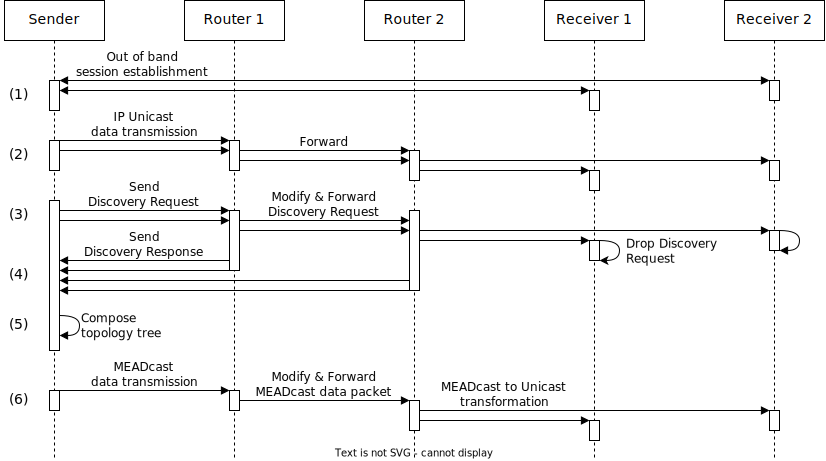
\includegraphics[width=.95\textwidth]{Bilder/mead_seq_dia.pdf}
    \caption{Interaction among participants in a MEADcast session (based on
        \cite{meadcast2})}
    \label{fig:mead_seq_dia}
\end{figure}

\begin{figure}
\centering
\begin{forest}
    for tree={grow=east, circle, draw, font=\footnotesize, l sep=14ex},
        where level=0{minimum size=2em}{},
        where level=2{
            s sep+=36pt
        }{},
        where level=4{l sep-=40}{},
        where={n_children==0}{font=\scriptsize, edge=dashed}{}
    [$S$
        [$R_1$,
            edge label={node[midway,above=3mm,font=\tiny,align=center]{
                Unicast: \{$E_1$\}\\
                \{$\underline{R_6}$,$E_2$,$E_3$,$\underline{R_7}$,$E_4$,$E_5$\}
            }}
            [$R_2$,
            edge label={node[midway,above=3mm,font=\tiny,align=center]{
                Unicast: \{$E_1$\}\\
                \{$\underline{R_6}$,$E_2$,$E_3$,$\underline{\cancel{R_7}}$,
                    $\cancel{E_4}$,$\cancel{E_5}$\}\\
                \{$\underline{\cancel{R_6}}$,$\cancel{E_2}$,$\cancel{E_3}$,
                    $\underline{R_7}$,$E_4$,$E_5$\}
            }}
                [$R_4$,
            edge label={node[midway,above,sloped,font=\tiny,align=left]{
                \{$\underline{R_6}$,$E_2$,$E_3$,$\underline{\cancel{R_7}}$,
                    $\cancel{E_4}$,$\cancel{E_5}$\}\\
                \{$\underline{\cancel{R_6}}$,$\cancel{E_2}$,$\cancel{E_3}$,
                    $\underline{R_7}$,$E_4$,$E_5$\}
            }}
                    [$R_7$,
                        edge label={node[midway,below=2mm,sloped,font=\tiny,align=center]{
                            \{$\underline{\cancel{R_6}}$,$\cancel{E_2}$,$\cancel{E_3}$,
                                $\underline{R_7}$,$E_4$,$E_5$\}
                        }}
                        [$E_5$,
                            edge label={node[midway,above=1mm,align=center,font=\tiny]{unicast}}
                        ][$E_4$]
                    ]
                    [$R_6$,
                        edge label={node[midway,above,sloped,font=\tiny,align=center]{
                            \{$\underline{R_6}$,$E_2$,$E_3$,$\underline{\cancel{R_7}}$,
                                $\cancel{E_4}$,$\cancel{E_5}$\}\\
                        }}
                        [$E_3$,
                            edge label={node[midway,above=1mm,align=center,font=\tiny]{unicast}}
                        ][$E_2$]
                    ]
                ]
                [$R_3$,
                    edge label={node[midway,above,sloped,font=\tiny,align=center]{
                        Unicast: \{$E_1$\}
                    }}
                    [$E_1$,
                        edge label={node[midway,above,align=center,font=\tiny]{unicast}}
                    ]
                ]
            ]
        ]
    ]
\end{forest}
\caption{MEADcast data delivery}
\label{fig:mead_delivery}
\end{figure}

% subsection MEADcast (end)
% section Mutlicast (end)

\section{Linux Kernel} % (fold)
\label{sec:Linux Kernel}

\subsection{Fundamentals} % (fold)
\label{sub:Fundamentals}

% subsection Fundamentals (end)

\subsection{Network Stack} % (fold)
\label{sub:Network Stack}

% subsection Network Stack (end)
% section Linux Kernel Network Internals (end)

% chapter Background Work (end)
